\chapter{Architettura del Sistema e Metodologia}
\label{cap:architettura_sistema_metodologia}

Questo capitolo descrive l'architettura del sistema sviluppato e la metodologia adottata per il confronto tra modelli di classificazione classici e quantistici. Vengono presentati, in ordine: l'architettura generale del sistema e il flusso di elaborazione dei dati; lo stack tecnologico e l'ambiente di sviluppo, incluso l'utilizzo di container Docker per garantire la riproducibilità dell'ambiente sperimentale; i dataset reali selezionati e le relative fasi di preprocessing; i principi di progettazione dei circuiti quantistici utilizzati come feature map e come ansatz variazionale; l'ambiente di esecuzione, distinto tra simulazione locale ed esecuzione su hardware quantistico reale; infine, il protocollo sperimentale e le metriche adottate per la valutazione comparativa dei modelli. Gli aspetti implementativi, incluso il codice sorgente sviluppato, sono rimandati al Capitolo~\ref{cap:implementazione_sperimentale_risultati} (Implementazione Sperimentale e Risultati).

\section{Architettura generale del sistema}
\label{sec:architettura_generale}

Il sistema è stato progettato secondo un'architettura modulare, in cui ciascuna fase della pipeline sperimentale è isolata in un componente distinto e riutilizzabile. Questa scelta progettuale persegue tre obiettivi principali: favorire la manutenibilità del codice, consentire il confronto sistematico tra modelli classici e quantistici a parità di dati in ingresso, e permettere l'estensione del sistema a nuovi dataset o a nuove architetture di circuito senza dover modificare le fasi precedenti della pipeline.

L'architettura complessiva può essere suddivisa nei seguenti moduli logici:

\begin{enumerate}
    \item \textbf{Modulo di acquisizione dei dati}: si occupa del caricamento dei dataset dalle librerie standard (Scikit-learn) e dalla loro validazione preliminare (verifica di valori mancanti, tipi di dato, bilanciamento delle classi).
    \item \textbf{Modulo di preprocessing}: applica la normalizzazione Min-Max e, dove necessario, la riduzione della dimensionalità tramite Analisi delle Componenti Principali (PCA), producendo in uscita un insieme di feature compatibile sia con i classificatori classici sia con il numero di qubit disponibili per i circuiti quantistici.
    \item \textbf{Modulo di codifica quantistica}: Converte i vettori dei dati pre-elaborati in circuiti quantistici parametrizzati (mappa delle caratteristiche), in accordo con i due metodi indicati nella Sezione~\ref{sec:circuiti_quantistici}.
    \item \textbf{Modulo di addestramento}: Prevede sia algoritmi classici forniti da Scikit-learn per avere un punto di riferimento, che modelli quantistici come QSVC e VQC costruiti tramite qiskit-machine-learning.
    \item \textbf{Modulo di esecuzione}: Gestisce il trasferimento dei circuiti sul back end scelto che può essere sia un simulatore locale senza rumore, sia un simulatore con rumore, sia un dispositivo quantistico reale disponibile sulla IBM Quantum Platform.
    \item \textbf{Modulo di valutazione}: Calcola le metriche delle prestazioni (Sezione~\ref{sec:protocollo_sperimentale}) e genera il confronto tra i risultati ottenuti dai modelli classici e quantistici.
\end{enumerate}

Il flusso dei dati avviene attraverso questi moduli in sequenza ma l'architettura permette lo svolgimento autonomo di ogni singola fase e la memorizzazione degli stati intermedi (ad esempio i dati normalizzati).

\begin{figure}[htbp]
    \centering
    \begin{tikzpicture}[
        node distance=0.9cm and 1cm,
        modulo/.style={
            rectangle, draw=blue!60!black, thick, rounded corners=2pt,
            fill=blue!6, minimum width=3.1cm, minimum height=1.15cm,
            align=center, font=\small
        },
        freccia/.style={-{Latex[length=2.2mm, width=1.6mm]}, thick, blue!60!black}
    ]
        % Riga superiore: fasi 1-3
        \node[modulo] (acq)  {\textbf{1}. Acquisizione\\dei dati};
        \node[modulo, right=of acq] (pre)  {\textbf{2}. Preprocessing};
        \node[modulo, right=of pre] (cod)  {\textbf{3}. Codifica\\quantistica};

        % Riga inferiore: fasi 4-6 (percorso a serpentina)
        \node[modulo, below=of cod]  (add)  {\textbf{4}. Addestramento};
        \node[modulo, left=of add]   (esec) {\textbf{5}. Esecuzione};
        \node[modulo, left=of esec]  (val)  {\textbf{6}. Valutazione};

        % Frecce di flusso dati
        \draw[freccia] (acq) -- (pre);
        \draw[freccia] (pre) -- (cod);
        \draw[freccia] (cod) -- (add);
        \draw[freccia] (add) -- (esec);
        \draw[freccia] (esec) -- (val);

        % Cornice che racchiude l'intera pipeline
        \begin{scope}[on background layer]
            \node[draw=gray!50, dashed, rounded corners=4pt,
                  fit=(acq)(pre)(cod)(add)(esec)(val),
                  inner sep=10pt, label={[gray!70, font=\scriptsize]above left:Pipeline sperimentale}] {};
        \end{scope}
    \end{tikzpicture}
    \caption{Schema a blocchi dell'architettura complessiva del sistema.}
    \label{fig:architettura_blocchi}
\end{figure}

Questa organizzazione modulare riflette anche la struttura del codice sorgente e dell'ambiente containerizzato descritto nella Sezione~\ref{sec:docker}, in cui ciascun modulo corrisponde a un insieme distinto di notebook Jupyter e script Python.

\section{Stack tecnologico e ambiente di sviluppo}
\label{sec:workflow_complessivo}

L'intero sistema si basa su un workflow strutturato che permette di addestrare e valutare modelli di machine learning quantistico utilizzando il framework Qiskit\footnote{Qiskit contributors. (2019). \textit{Qiskit: An Open-Source Framework for Quantum Computing}. Zenodo. \url{https://doi.org/10.5281/zenodo.2562111}.}. Il workflow complessivo comprende diverse fasi: raccolta e preparazione dei dati, preprocessing, addestramento del modello quantistico, valutazione delle performance e confronto con modelli classici. Tutte le fasi sono implementate utilizzando Python e librerie standard del data science, eseguite all'interno di un ambiente containerizzato per garantire la riproducibilità dei risultati.

\subsection{Python e librerie scientifiche di base}
Python è il linguaggio principale utilizzato per lo sviluppo del sistema, grazie alla sua sintassi semplice e alla disponibilità di librerie specializzate per la data science.
Per lo sviluppo viene utilizzato l'ambiente Jupyter Notebook\footnote{Kluyver, T., Ragan-Kelley, B., Pérez, F., Granger, B., Bussonnier, M., Frederic, J., Kelley, K., Hamrick, J., Grout, J., Corlay, S., Ivanov, P., Avila, D., Abdalla, S., \& Willing, C. (2016). Jupyter Notebooks -- a publishing format for reproducible computational workflows. In F. Loizides \& B. Schmidt (a cura di), \textit{Positioning and Power in Academic Publishing: Players, Agents and Agendas} (pp. 87--90). IOS Press. \url{https://doi.org/10.3233/978-1-61499-649-1-87}. Documentazione ufficiale del progetto Jupyter: \url{https://jupyter.org}.}, che consente una sperimentazione interattiva e una facile visualizzazione dei risultati intermedi. Le librerie di base utilizzate appartengono allo stack scientifico standard di Python:

\begin{itemize}
    \item \textbf{NumPy}\footnote{Harris, C. R., Millman, K. J., van der Walt, S. J., Gommers, R., Virtanen, P., Cournapeau, D., Wieser, E., Taylor, J., Berg, S., Smith, N. J., Kern, R., Picus, M., Hoyer, S., van Kerkwijk, M. H., Brett, M., Haldane, A., Fernández del Río, J., Wiebe, M., Peterson, P., Gérard-Marchant, P., Sheppard, K., Reddy, T., Weckesser, W., Abbasi, H., Gohlke, C., \& Oliphant, T. E. (2020). Array programming with NumPy. \textit{Nature}, 585(7825), 357--362. \url{https://doi.org/10.1038/s41586-020-2649-2}. Documentazione ufficiale: \url{https://numpy.org}.}: essenziale per la gestione delle operazioni matematiche e dei vettori multidimensionali. Viene utilizzato per la rappresentazione interna dei dati e per le operazioni di base necessarie all'addestramento dei modelli.
    \item \textbf{Pandas}\footnote{McKinney, W. (2010). Data Structures for Statistical Computing in Python. In S. van der Walt \& J. Millman (a cura di), \textit{Proceedings of the 9th Python in Science Conference} (pp. 56--61). \url{https://doi.org/10.25080/Majora-92bf1922-00a}. Documentazione ufficiale: \url{https://pandas.pydata.org}.}: offre strumenti per l'analisi e la manipolazione dei dati strutturati, permettendo una gestione efficiente dei dataset prima dell'addestramento dei modelli quantistici.
    \item \textbf{Matplotlib}\footnote{Hunter, J. D. (2007). Matplotlib: A 2D Graphics Environment. \textit{Computing in Science \& Engineering}, 9(3), 90--95. \url{https://doi.org/10.1109/MCSE.2007.55}. Documentazione ufficiale: \url{https://matplotlib.org}.} \textbf{e Seaborn}\footnote{Waskom, M. L. (2021). seaborn: statistical data visualization. \textit{Journal of Open Source Software}, 6(60), 3021. \url{https://doi.org/10.21105/joss.03021}. Documentazione ufficiale: \url{https://seaborn.pydata.org}.}: librerie per la visualizzazione dei dati, utilizzate per analizzare i risultati e le performance dei modelli.
\end{itemize}

La scelta di Python deriva dalla sua natura versatile e dalla sua adattabilità alle esigenze del machine learning quantistico, inclusa la possibilità di integrare facilmente librerie specifiche per la computazione quantistica.

\subsection{Containerizzazione dell'ambiente con Docker}
\label{sec:docker}

Uno degli aspetti metodologici centrali del presente lavoro è la riproducibilità dell'ambiente sperimentale. Le librerie di calcolo quantistico, in particolare Qiskit e qiskit-machine-learning, sono soggette a un ritmo di aggiornamento rapido, con frequenti modifiche alle interfacce pubbliche tra una versione e l'altra. Per evitare che risultati e comportamento del sistema dipendano dalla specifica combinazione di versioni installate sulla macchina di sviluppo, l'intero ambiente è stato containerizzato utilizzando Docker\footnote{Merkel, D. (2014). Docker: Lightweight Linux Containers for Consistent Development and Deployment. \textit{Linux Journal}, 2014(239), Articolo 2. Documentazione ufficiale: \url{https://docs.docker.com}.} e orchestrato tramite Docker Compose\footnote{Documentazione ufficiale: \url{https://docs.docker.com/compose/}.}.

\subsubsection{Motivazioni della scelta}
L'adozione di un ambiente containerizzato risponde a diverse esigenze metodologiche:
\begin{itemize}
    \item \textbf{Riproducibilità}: fissare le versioni di Python, Qiskit, Scikit-learn e delle altre dipendenze garantisce che i risultati sperimentali riportati in questa tesi siano riproducibili in futuro, anche a fronte di aggiornamenti delle librerie utilizzate.
    \item \textbf{Isolamento}: il container isola l'ambiente di sviluppo dal sistema operativo host, evitando conflitti tra dipendenze di progetti diversi e semplificando la gestione delle versioni.
    \item \textbf{Portabilità}: l'ambiente può essere eseguito in modo identico su macchine diverse (ad esempio la workstation utilizzata per lo sviluppo e un eventuale server con maggiore capacità di calcolo), senza necessità di reinstallare manualmente le dipendenze.
    \item \textbf{Documentazione implicita}: il file \texttt{Dockerfile} e il file \texttt{docker-compose.yml} costituiscono essi stessi una descrizione precisa e verificabile dell'ambiente utilizzato, riducendo l'ambiguità tipica delle descrizioni testuali degli ambienti software.
\end{itemize}

\subsubsection{Struttura dell'ambiente containerizzato}
L'ambiente è organizzato secondo l'approccio standard di Docker, basato su due file di configurazione distinti e complementari, il cui contenuto dettagliato (incluso il codice) è riportato nel Capitolo~\ref{cap:implementazione_sperimentale_risultati}:

\begin{itemize}
    \item Il \textbf{Dockerfile} definisce l'immagine di base del container, a partire da un'immagine Python ufficiale con versione fissata, e specifica il processo di costruzione dell'ambiente: installazione delle dipendenze di sistema necessarie, installazione delle librerie Python elencate in un file dei requisiti con versioni fissate (\textit{pinning}), configurazione dell'utente di esecuzione e della directory di lavoro, ed esposizione della porta utilizzata dal server Jupyter.
    \item Il file \textbf{docker-compose.yml} orchestra il servizio definito dal Dockerfile, specificando: il montaggio della directory del progetto come volume, in modo da rendere persistenti i notebook e i dati anche dopo l'arresto del container; la mappatura delle porte tra host e container per l'accesso all'interfaccia Jupyter; le eventuali variabili d'ambiente necessarie per l'autenticazione ai servizi di IBM Quantum Platform (Sezione~\ref{sec:esecuzione_hardware_reale}); i limiti di risorse computazionali assegnate al container, ove rilevanti per le simulazioni più onerose.
\end{itemize}

Questa configurazione consente di avviare l'intero ambiente di sviluppo con un singolo comando, garantendo che chiunque esegua nuovamente gli esperimenti disponga esattamente delle stesse versioni di librerie utilizzate in fase di sviluppo. La scelta di separare la definizione dell'immagine (Dockerfile) dall'orchestrazione del servizio (docker-compose.yml) segue le pratiche raccomandate per progetti di ricerca riproducibili, e consente in prospettiva di estendere l'architettura con servizi aggiuntivi (ad esempio un servizio dedicato al tracciamento degli esperimenti) senza modificare l'immagine di base.

\begin{figure}[htbp]
    \centering
    \begin{tikzpicture}[
        comp/.style={
            rectangle, draw=blue!60!black, thick, rounded corners=2pt,
            fill=blue!6, minimum width=4cm, minimum height=0.95cm,
            align=center, font=\small
        },
        vol/.style={
            rectangle, draw=orange!70!black, thick, rounded corners=2pt,
            fill=orange!8, minimum width=3.6cm, minimum height=0.95cm,
            align=center, font=\small
        },
        porta/.style={
            rectangle, draw=violet!60!black, thick, rounded corners=2pt,
            fill=violet!6, minimum width=3.6cm, minimum height=0.85cm,
            align=center, font=\small
        },
        freccia/.style={-{Latex[length=2.2mm, width=1.5mm]}, thick},
        etichetta/.style={font=\scriptsize, align=center}
    ]

        % --- Colonna host (sinistra) ---
        \node[porta] (portahost) at (0, 1.4) {Browser\\\texttt{localhost:8888}};
        \node[vol]   (progetto)  at (0, -1.4) {Folders\\\texttt{./notebooks}, \texttt{./src}, \texttt{./data}};

        % --- Colonna container (destra) ---
        \node[comp] (jupyter) at (6.0, 1.4)  {Server Jupyter\\(porta 8888)};
        \node[comp] (workdir) at (6.0, 0)     {Volume montato\\\texttt{\textasciitilde/projects/thesis}};
        \node[comp] (qiskit)  at (6.0, -1.4) {Python + Qiskit SDK\\+ qiskit-machine-learning};

        % --- Riquadri di raggruppamento ---
        \begin{scope}[on background layer]
            \node[draw=gray!60, dotted, rounded corners=4pt,
                  fit=(portahost)(progetto), inner sep=10pt,
                  label={[gray!60, font=\small\bfseries, label distance=3pt]above:Macchina host}] (hostbox) {};
            \node[draw=blue!50!black, dashed, rounded corners=4pt,
                  fit=(jupyter)(workdir)(qiskit), inner sep=10pt,
                  label={[blue!50!black, font=\small\bfseries, label distance=3pt]above:Container Docker}] (containerbox) {};
        \end{scope}

        % --- Frecce ---
        \draw[freccia, violet!60!black, <->] (portahost) -- node[etichetta, above]{mappatura porta\\\texttt{8888:8888}} (jupyter);
        \draw[freccia, orange!70!black, <->] (progetto) -- node[etichetta, above]{bind mount\\(volume)} (workdir);

    \end{tikzpicture}
    \caption{Schema dell'ambiente di sviluppo containerizzato basato su Docker Compose.}
    \label{fig:docker_architettura}
\end{figure}

\subsection{Scikit-learn}
Scikit-learn\footnote{Pedregosa, F., Varoquaux, G., Gramfort, A., Michel, V., Thirion, B., Grisel, O., Blondel, M., Prettenhofer, P., Weiss, R., Dubourg, V., Vanderplas, J., Passos, A., Cournapeau, D., Brucher, M., Perrot, M., \& Duchesnay, E. (2011). Scikit-learn: Machine Learning in Python. \textit{Journal of Machine Learning Research}, 12, 2825--2830.} è una libreria fondamentale per l'implementazione di algoritmi di machine learning classici. Nel presente lavoro è utilizzata principalmente come baseline per il confronto con i modelli quantistici. Essa offre una grande varietà di algoritmi, tra cui:
\begin{itemize}
    \item Classificatori: Logistic Regression, Decision Tree, Random Forest, Support Vector Machine (SVM)
    \item Tecniche di preprocessing: \texttt{StandardScaler}, \texttt{MinMaxScaler}
    \item Tecniche di riduzione della dimensionalità: \texttt{PCA}
    \item Metriche di valutazione: accuratezza, precisione, richiamo (\textit{recall}), F1-score
\end{itemize}

La scelta di Scikit-learn deriva dalla sua semplicità d'uso, dalla documentazione completa e dall'ampia comunità di sviluppatori che la utilizza sia in ambito accademico sia industriale, il che la rende uno standard \textit{de facto} per il confronto tra algoritmi di classificazione.

\subsection{Qiskit SDK}
Il framework Qiskit\footnote{Qiskit contributors. (2019). \textit{Qiskit: An Open-Source Framework for Quantum Computing}. Zenodo. \url{https://doi.org/10.5281/zenodo.2562111}.} rappresenta il nucleo tecnologico del sistema per quanto riguarda la componente quantistica. È un SDK open source per la programmazione quantistica che consente la costruzione, la trasformazione e l'esecuzione di circuiti quantistici. Le componenti principali di Qiskit rilevanti per questo lavoro includono:

\begin{itemize}
    \item \textbf{Qiskit SDK (core)}: fornisce le astrazioni di base per la costruzione e l'ottimizzazione dei circuiti quantistici (oggetto \texttt{QuantumCircuit}), le primitive di riferimento \texttt{StatevectorSampler} e \texttt{StatevectorEstimator} per la simulazione locale ideale, e il transpiler per l'adattamento dei circuiti ai vincoli topologici e al set di porte di uno specifico backend.
    \item \textbf{Qiskit Aer}\footnote{\url{https://qiskit.github.io/qiskit-aer/}.}: simulatore avanzato di circuiti quantistici che consente l'esecuzione locale di modelli complessi, incluse simulazioni con modelli di rumore realistici.
    \item \textbf{Qiskit Runtime}\footnote{\url{https://quantum.cloud.ibm.com/docs}.}: ambiente di esecuzione che fornisce le implementazioni ottimizzate delle primitive \texttt{Sampler} ed \texttt{Estimator} per l'esecuzione su hardware quantistico reale tramite IBM Quantum Platform, come descritto nella Sezione~\ref{sec:esecuzione_hardware_reale}.
    \item \textbf{qiskit-machine-learning}: libreria che fornisce implementazioni specifiche per il machine learning quantistico, descritta in dettaglio nella sottosezione seguente.
\end{itemize}

L'utilizzo di Qiskit permette non solo di implementare i modelli quantistici, ma anche di eseguirli su backend differenti, che vanno dalla simulazione locale ideale ai computer quantistici reali, mantenendo la medesima interfaccia di programmazione basata sulle primitive \texttt{Sampler} ed \texttt{Estimator}. Questo permette di effettuare un ciclo di sviluppo e validazione dei modelli progressivo, come descritto nella Sezione~\ref{sec:strategia_valutazione}.

\subsection{qiskit-machine-learning}
\label{sec:qiskit_machine_learning}
La libreria qiskit-machine-learning è la componente specifica per il machine learning quantistico costruita sopra il Qiskit SDK. Nel contesto di questo lavoro fornisce:
\begin{itemize}
    \item Implementazioni di \textbf{QSVC} (\textit{Quantum Support Vector Classifier}) e \textbf{VQC} (\textit{Variational Quantum Classifier}), descritti nella Sezione~\ref{sec:circuiti_quantistici};
    \item Kernel quantistici (\textit{quantum kernels}) per il calcolo delle similarità tra i dati nello spazio di Hilbert indotto dalla feature map;
    \item Feature map parametriche per la trasformazione dei dati classici in stati quantistici;
    \item Interfacce verso ottimizzatori classici (ad esempio COBYLA e SPSA) per l'aggiornamento dei parametri variazionali dei modelli quantistici.
\end{itemize}

Questa libreria si basa sui principi fondamentali introdotti nel Qiskit SDK e permette di creare un modello quantistico completo senza la necessità di gestire manualmente tutti i dettagli a livello di porte logiche quantistiche, al tempo stesso garantendo un controllo preciso sulla struttura del circuito.

\subsection{Ambiente Jupyter e Workflow di Sviluppo}
Il workflow è organizzato in modo da consentire un facile riutilizzo del codice, una documentazione chiara e un confronto sistematico tra i modelli quantistici e classici.
Le fasi principali, che rispecchiano i moduli architetturali descritti nella Sezione~\ref{sec:architettura_generale}, sono:

\begin{enumerate}
    \item \textbf{Raccolta e preparazione dei dati}: selezione dei dataset, verifica dell'integrità e adattamento al formato richiesto dalle fasi successive.
    \item \textbf{Preprocessing}: normalizzazione, riduzione della dimensionalità e generazione dei vettori di input per i circuiti quantistici.
    \item \textbf{Costruzione del modello}: scelta della struttura del circuito quantistico (feature map e, per il VQC, ansatz variazionale).
    \item \textbf{Addestramento del modello}: utilizzo di ottimizzatori classici per l'addestramento dei parametri quantistici, oppure addestramento diretto per i modelli classici di confronto.
    \item \textbf{Valutazione}: misurazione delle prestazioni utilizzando le metriche menzionate nella Sezione~\ref{sec:protocollo_sperimentale} e confronto sistematico con i modelli classici.
    \item \textbf{Analisi dei risultati}: Analisi delle prestazioni di ogni modello e discussione dei punti di forza e degli eventuali limiti.
\end{enumerate}

Con questo approccio modulare è infatti possibile valutare rapidamente diverse configurazioni per trovare quelle più adatte in base alle peculiarità dei dati e del problema che si vuole risolvere senza dover riscrivere le fasi comuni della pipeline.

\section{Dataset reali e preprocessing}
\label{sec:dataset_preprocessing}

Per l'implementazione e la valutazione dei modelli quantistici è stato utilizzato un insieme di dataset reali, resi disponibili tramite Scikit-learn. La scelta dei dataset è stata guidata dal vincolo per cui i modelli quantistici implementabili su simulatore e su hardware attuale richiedono un numero ridotto di feature (indicativamente 4-8 qubit) e un numero contenuto di campioni, per motivi di efficienza computazionale sia in fase di simulazione sia in fase di esecuzione su hardware reale, dove i tempi di coda e il costo computazionale crescono rapidamente con la dimensione del problema.

\subsection{Criteri di selezione dei dataset}
Sono stati selezionati tre dataset riconosciuti in letteratura per la loro utilità nel contesto della classificazione supervisionata. La scelta è stata guidata da diversi fattori:
\begin{itemize}
    \item \textbf{Natura numerica delle feature}: tutti i dataset selezionati presentano feature numeriche continue, direttamente compatibili con le porte di rotazione parametriche (RX, RY, RZ) utilizzate nelle feature map quantistiche.
    \item \textbf{Dimensionalità}: i dataset presentano dimensionalità differenti (da 13 a 64 feature originarie), permettendo di valutare l'effetto della riduzione dimensionale sulle performance dei modelli.
    \item \textbf{Tipo di problema}: sono rappresentati sia problemi di classificazione binaria sia multiclasse, per garantire una valutazione comparativa più ampia.
    \item \textbf{Accessibilità e riproducibilità}: tutti i dataset sono disponibili pubblicamente tramite Scikit-learn e provengono da fonti citabili e verificabili (UCI Machine Learning Repository), condizione necessaria per garantire la riproducibilità degli esperimenti.
\end{itemize}

\subsection{Dataset selezionati}

\subsubsection{Breast Cancer Wisconsin}
Il dataset \textit{Breast Cancer Wisconsin (Diagnostic)}\footnote{Wolberg, W., Street, W., \& Mangasarian, O. (1995). \textit{Breast Cancer Wisconsin (Diagnostic)} [Dataset]. UCI Machine Learning Repository. \url{https://archive.ics.uci.edu/dataset/17/breast-cancer-wisconsin-diagnostic}.} è uno dei dataset più utilizzati in letteratura per problemi di classificazione binaria in ambito medico, e rappresenta un insieme di 569 campioni con 30 feature. Ogni feature descrive una caratteristica geometrica o di texture dei nuclei cellulari, ottenute dall'analisi digitale di un'immagine di agoaspirato di massa mammaria (\textit{Fine Needle Aspirate}, FNA). Il dataset è ritenuto adatto per la sperimentazione con il machine learning quantistico per i seguenti motivi:
\begin{itemize}
    \item le feature sono tutte numeriche e continue, adatte alla codifica su porte di rotazione quantistiche;
    \item il problema è binario (tumore benigno o maligno), semplice da interpretare e ben studiato in letteratura come benchmark;
    \item la dimensionalità originaria (30 feature) è elevata rispetto al numero di qubit tipicamente disponibili, rendendo necessaria una riduzione della dimensionalità (Sezione~\ref{sec:pca});
    \item la distribuzione delle classi (357 campioni benigni e 212 maligni) non è fortemente sbilanciata, pur presentando una moderata asimmetria di cui si tiene conto nella scelta delle metriche di valutazione (Sezione~\ref{sec:protocollo_sperimentale}).
\end{itemize}

\subsubsection{Wine}
Il dataset \textit{Wine}\footnote{Aeberhard, S., \& Forina, M. (1992). \textit{Wine} [Dataset]. UCI Machine Learning Repository. \url{https://doi.org/10.24432/C5PC7J}.} contiene 178 campioni con 13 feature che rappresentano proprietà chimiche e fisiche di vini appartenenti a tre diversi cultivar, coltivati nella medesima regione italiana. Questo dataset è adatto alla classificazione multiclasse e presenta diversi vantaggi:
\begin{itemize}
    \item le feature sono tutte numeriche e continue;
    \item le classi sono relativamente bilanciate (59, 71 e 48 campioni rispettivamente per i tre cultivar);
    \item consente l'analisi di un problema multiclasse a tre categorie, più complesso rispetto al caso binario;
    \item la dimensionalità originaria (13 feature) è già contenuta, richiedendo una riduzione dimensionale meno aggressiva rispetto agli altri dataset selezionati.
\end{itemize}

\subsubsection{Digits}
Il dataset \textit{Optical Recognition of Handwritten Digits}\footnote{Alpaydin, E., \& Kaynak, C. (1998). \textit{Optical Recognition of Handwritten Digits} [Dataset]. UCI Machine Learning Repository. \url{https://doi.org/10.24432/C50P49}.}, comunemente noto come \textit{Digits} nell'implementazione di Scikit-learn, contiene immagini di cifre scritte a mano, rappresentate come matrici di 8$\times$8 pixel (64 feature totali). Ogni elemento della matrice rappresenta il livello di grigio del pixel corrispondente, codificato come intero compreso tra 0 e 16. Questo dataset rappresenta un problema classico di riconoscimento di immagini e presenta le seguenti caratteristiche:
\begin{itemize}
    \item ogni cifra è rappresentata da 64 feature (matrice 8$\times$8 di pixel);
    \item le classi sono 10, corrispondenti alle cifre da 0 a 9;
    \item è un problema di classificazione multiclasse ben definito e ampiamente utilizzato come benchmark;
    \item la dimensionalità è la più elevata tra i dataset selezionati, rendendo la riduzione dimensionale un passaggio essenziale piuttosto che opzionale.
\end{itemize}

I tre dataset sono stati scelti congiuntamente perché, pur condividendo la natura numerica delle feature e problemi di classificazione ben formulati, si distinguono per condizioni sperimentali diverse: classificazione binaria e multiclasse, dimensionalità bassa, media e alta, e campi di applicazione differenti (diagnosi mediche, chimica analitica, visione artificiale).

\subsection{Preelaborazione e Normalizzazione}
Le fasi di pre-elaborazione sono necessarie per rendere i dataset compatibili con i requisiti dell'apprendimento quantistico.
La normalizzazione dei dati è in particolare necessaria per garantire la stabilità dell'addestramento e la corretta interpretazione dei valori delle feature come angoli di rotazione nei circuiti quantistici.

La normalizzazione è effettuata con l'approccio Min-Max, che trasforma i valori di ciascuna feature in un intervallo compreso tra 0 e 1:

\begin{equation}
x_{norm} = \frac{x - x_{min}}{x_{max} - x_{min}}
\end{equation}

Questa normalizzazione è necessaria perché le feature map quantistiche utilizzate impiegano porte di rotazione (RX, RY, RZ) i cui angoli dipendono dai valori delle feature in ingresso; un intervallo limitato e uniforme è pertanto opportuno per evitare rotazioni eccessive che comprometterebbero la distinguibilità degli stati quantistici codificati.
La scelta di questa strategia rispetto ad altre strategie come la normalizzazione dello z-score è dovuta alle seguenti ragioni:

\begin{itemize}
    \item facilità di interpretazione e implementazione;
    \item Compatibilità con la formalizzazione delle porte di rotazione quantistiche che funzionano intrinsecamente su un intervallo finito di angoli;
    \item Un comportamento di addestramento più stabile che è stato osservato empiricamente nelle fasi iniziali degli esperimenti;
    \item Coerenza nella rappresentazione dei dati indipendentemente dalla scala delle singole caratteristiche.
\end{itemize}

È opportuno segnalare che la normalizzazione Min-Max, calcolata sui valori minimo e massimo osservati, deve essere derivata esclusivamente dal set di addestramento e successivamente applicata al set di test, per evitare fenomeni di \textit{data leakage} che comprometterebbero la validità della valutazione (si veda la Sezione~\ref{sec:protocollo_sperimentale}).

\subsection{Riduzione della dimensionalità tramite PCA}
\label{sec:pca}
Poiché il numero di qubit disponibili, sia in simulazione sia su hardware reale, è limitato, è necessario ridurre la dimensionalità dei dataset con dimensionalità originaria elevata mediante l'Analisi delle Componenti Principali (\textit{Principal Component Analysis}, PCA)\footnote{Jolliffe, I. T. (2002). \textit{Principal Component Analysis} (2nd ed.). Springer Series in Statistics. Springer.}.
La necessità di una tale riduzione nasce da:
\begin{itemize}
    \item l'adattamento dei dati al formato del circuito quantistico dove ogni caratteristica viene normalmente mappata su un qubit dedicato;
    \item la garanzia della conservazione di schemi essenziali all'interno del set di dati garantendo al contempo una minima perdita di informazioni discriminanti tra le classi;
    \item la riduzione del tempo di calcolo impiegato durante l'addestramento sia attraverso la simulazione che l'esecuzione effettiva;
    \item la combinazione delle caratteristiche originali per formare un numero minore di componenti da memorizzare su un numero ridotto di qubit.
\end{itemize}

Il processo di riduzione si basa sull'analisi della varianza spiegata da ciascuna componente principale.
Vengono selezionate le componenti che rappresentano complessivamente una percentuale significativa della varianza totale del dataset, individuata tramite l'analisi del grafico della varianza cumulata (\textit{scree plot}).

\begin{figure}[htbp]
    \centering
    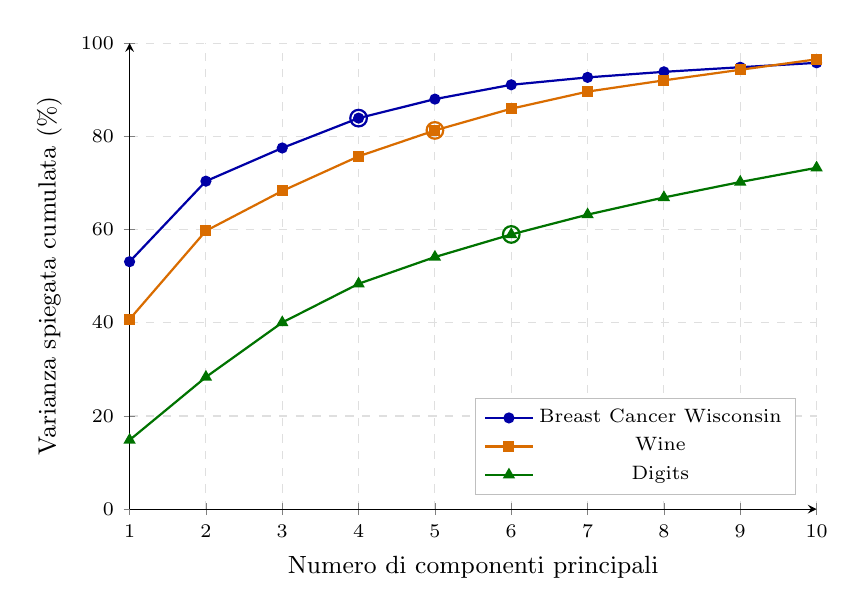
\begin{tikzpicture}
        \begin{axis}[
            width=0.85\textwidth,
            height=7.5cm,
            xlabel={Numero di componenti principali},
            ylabel={Varianza spiegata cumulata (\%)},
            xmin=1, xmax=10,
            ymin=0, ymax=100,
            xtick={1,2,3,4,5,6,7,8,9,10},
            ytick={0,20,40,60,80,100},
            grid=major,
            grid style={dashed, gray!25},
            legend pos=south east,
            legend style={font=\scriptsize, draw=gray!50},
            axis lines=left,
            tick label style={font=\scriptsize},
            label style={font=\small},
        ]

        % --- Breast Cancer Wisconsin ---
        \addplot[
            color=blue!65!black, mark=*, mark size=1.6pt, thick
        ] coordinates {
            (1,53.10) (2,70.38) (3,77.50) (4,83.91) (5,87.99)
            (6,91.06) (7,92.65) (8,93.84) (9,94.83) (10,95.77)
        };
        \addlegendentry{Breast Cancer Wisconsin}

        % --- Wine ---
        \addplot[
            color=orange!85!black, mark=square*, mark size=1.6pt, thick
        ] coordinates {
            (1,40.75) (2,59.72) (3,68.28) (4,75.71) (5,81.27)
            (6,85.93) (7,89.60) (8,92.01) (9,94.28) (10,96.53)
        };
        \addlegendentry{Wine}

        % --- Digits ---
        \addplot[
            color=green!45!black, mark=triangle*, mark size=1.8pt, thick
        ] coordinates {
            (1,14.82) (2,28.34) (3,40.05) (4,48.36) (5,54.10)
            (6,58.95) (7,63.20) (8,66.88) (9,70.20) (10,73.25)
        };
        \addlegendentry{Digits}

        % --- Marcatori delle componenti selezionate (Sezione 4.3.1) ---
        \addplot[color=blue!65!black, mark=o, mark size=3pt, only marks, thick] coordinates {(4,83.91)};
        \addplot[color=orange!85!black, mark=o, mark size=3pt, only marks, thick] coordinates {(5,81.27)};
        \addplot[color=green!45!black, mark=o, mark size=3pt, only marks, thick] coordinates {(6,58.95)};

        \end{axis}
    \end{tikzpicture}
    \caption{Varianza spiegata cumulata in funzione del numero di componenti principali per i dataset Breast Cancer Wisconsin, Wine e Digits. I marcatori cerchiati indicano il numero di componenti effettivamente selezionato per ciascun dataset (rispettivamente 4, 5 e 6). Questa analisi esplorativa è condotta sull'intero dataset (normalizzato con Min-Max, senza suddivisione train/test), a scopo puramente illustrativo della scelta del numero di componenti; i valori di varianza spiegata cumulata riportati in Tabella~\ref{tab:pca_componenti} del Capitolo~\ref{cap:implementazione_sperimentale_risultati}, leggermente diversi da quelli qui mostrati, sono invece calcolati sulla PCA effettivamente utilizzata dalla pipeline sperimentale, fittata esclusivamente sull'insieme di addestramento per evitare \textit{data leakage} (Sezione~\ref{sec:protocollo_sperimentale}).}
    \label{fig:pca_scree_plot}
\end{figure}

\subsubsection{Applicazione specifica della PCA}
La PCA è stata applicata in modo da adattare i dati alle capacità dei modelli quantistici implementati, tenendo conto sia della varianza spiegata sia del vincolo pratico sul numero massimo di qubit gestibile in simulazione:
\begin{itemize}
    \item per il dataset Breast Cancer Wisconsin sono state selezionate 4 componenti principali, che consentono di rappresentare una quota elevata della varianza complessiva pur mantenendo il numero di qubit ridotto;
    \item per il dataset Wine sono state utilizzate 5 componenti principali, sufficienti a coprire la maggior parte della varianza data la dimensionalità originaria contenuta del dataset;
    \item per il dataset Digits è stato fissato un limite massimo di 6 componenti principali, data l'elevata dimensionalità originaria (64 feature) e la necessità di contenere il numero di qubit richiesto.
\end{itemize}

Il numero definitivo di componenti per ciascun dataset è stato determinato attraverso un'analisi esplorativa della varianza cumulata, verificata empiricamente confrontando le performance dei modelli classici addestrati sulle feature ridotte rispetto a quelle ottenute sulle feature originarie; i risultati di tale analisi empirica sono riportati nel Capitolo~\ref{cap:implementazione_sperimentale_risultati}.

\subsubsection{Vantaggi e limiti della riduzione dimensionale}
L'uso della PCA in questo contesto presenta vantaggi e limitazioni che è opportuno esplicitare:
\begin{itemize}
    \item \textbf{Vantaggi}: riduce il numero di qubit necessari, preserva la maggior parte della varianza dei dati originari, facilita l'interpretabilità geometrica dello spazio delle feature risultante.
    \item \textbf{Limitazioni}: comporta la perdita delle informazioni associate alle componenti secondarie, che in alcuni casi potrebbero contenere segnale utile alla discriminazione tra classi; inoltre le componenti principali, essendo combinazioni lineari delle feature originarie, perdono in generale l'interpretabilità semantica diretta di queste ultime.
    \item \textbf{Effetto sulle performance}: la riduzione dimensionale rappresenta un compromesso tra fedeltà rispetto ai dati originari e fattibilità computazionale, spesso necessario per rendere trattabile l'addestramento dei modelli quantistici nell'orizzonte temporale e nelle risorse disponibili per questo lavoro.
\end{itemize}

La scelta del numero di componenti ha un impatto diretto sulle performance dei modelli quantistici implementati, e viene pertanto trattata anche come iperparametro sperimentale nel Capitolo~\ref{cap:implementazione_sperimentale_risultati}.

\section{Progettazione dei circuiti quantistici}
\label{sec:circuiti_quantistici}

La costruzione dei modelli di classificazione quantistica richiede la definizione di due elementi architetturali principali: la \textit{feature map}, responsabile della codifica dei dati classici in stati quantistici, e, nel caso del VQC, l'\textit{ansatz} variazionale, responsabile della parte addestrabile del circuito. Questa sezione ne descrive i principi metodologici; i dettagli implementativi e i parametri specifici utilizzati sono riportati nel capitolo successivo.

\subsection{Feature map: codifica dei dati classici in stati quantistici}
La feature map è un circuito quantistico parametrico $U_{\Phi(\mathbf{x})}$ che codifica un vettore di dati classici $\mathbf{x}$, ottenuto dopo normalizzazione e riduzione dimensionale, in uno stato quantistico $\ket{\Phi(\mathbf{x})} = U_{\Phi(\mathbf{x})}\ket{0}^{\otimes n}$, dove $n$ è il numero di qubit, tipicamente pari al numero di componenti principali selezionate per il dataset in esame. L'idea alla base di questo approccio, introdotta da Havlíček et al.\footnote{Havlíček, V., Córcoles, A. D., Temme, K., Harrow, A. W., Kandala, A., Chow, J. M., \& Gambetta, J. M. (2019). Supervised learning with quantum-enhanced feature spaces. \textit{Nature}, 567(7747), 209--212. \url{https://doi.org/10.1038/s41586-019-0980-2}.}, è che lo spazio di Hilbert esponenzialmente grande accessibile tramite un numero contenuto di qubit possa fungere da spazio delle feature arricchito, potenzialmente difficile da riprodurre in modo efficiente con un kernel classico.

Nel presente lavoro vengono impiegate feature map basate su porte di rotazione parametriche (RX, RY, RZ), i cui angoli sono determinati direttamente dai valori normalizzati delle feature, eventualmente combinate con porte di entanglement (ad esempio CNOT) per introdurre correlazioni tra qubit e quindi tra le feature codificate.

\begin{figure}[htbp]
    \centering
    \begin{quantikz}[row sep={0.7cm,between origins}, column sep=0.45cm]
        \lstick{$\ket{0}$} & \gate{H} & \gate{R_X(x_1)} & \ctrl{1} & \qw      & \qw      & \gate{R_Z(x_1)} & \qw \\
        \lstick{$\ket{0}$} & \gate{H} & \gate{R_X(x_2)} & \targ{}  & \ctrl{1} & \qw      & \gate{R_Z(x_2)} & \qw \\
        \lstick{$\ket{0}$} & \gate{H} & \gate{R_X(x_3)} & \qw      & \targ{}  & \ctrl{1} & \gate{R_Z(x_3)} & \qw \\
        \lstick{$\ket{0}$} & \gate{H} & \gate{R_X(x_4)} & \qw      & \qw      & \targ{}  & \gate{R_Z(x_4)} & \qw
    \end{quantikz}
    \caption{Esempio di circuito di codifica (feature map) a $n$ qubit.}
    \label{fig:feature_map_circuito}
\end{figure}

\subsection{Ansatz variazionale}
Per il modello VQC, oltre alla feature map è necessario definire un \textit{ansatz}: un circuito parametrico $V(\boldsymbol{\theta})$, i cui parametri $\boldsymbol{\theta}$ sono addestrabili tramite un ottimizzatore classico, applicato successivamente alla feature map. La struttura dell'ansatz determina l'espressività del modello, ovvero la varietà di funzioni di decisione che il circuito è in grado di rappresentare, ma influisce anche sulla difficoltà di addestramento, poiché ansatz eccessivamente espressivi sono più soggetti al fenomeno dei \textit{barren plateaus}, ovvero all'annullamento del gradiente della funzione di costo al crescere del numero di qubit e della profondità del circuito.

\begin{figure}[htbp]
    \centering
    \begin{quantikz}[row sep={0.7cm,between origins}, column sep=0.45cm]
        \lstick{$\ket{0}$} & \gate{R_Y(\theta_1)}\gategroup[4,steps=2,style={dashed,rounded corners,inner sep=6pt},label style={label position=above,anchor=south,yshift=0.2cm}]{{\footnotesize ripetuto $L$ volte}} & \ctrl{1} & \qw      & \qw      & \gate{R_Y(\theta_5)} & \qw \\
        \lstick{$\ket{0}$} & \gate{R_Y(\theta_2)} & \targ{}  & \ctrl{1} & \qw      & \gate{R_Y(\theta_6)} & \qw \\
        \lstick{$\ket{0}$} & \gate{R_Y(\theta_3)} & \qw      & \targ{}  & \ctrl{1} & \gate{R_Y(\theta_7)} & \qw \\
        \lstick{$\ket{0}$} & \gate{R_Y(\theta_4)} & \qw      & \qw      & \targ{}  & \gate{R_Y(\theta_8)} & \qw
    \end{quantikz}
    \caption{Esempio di circuito ansatz variazionale a $n$ qubit.}
    \label{fig:ansatz_circuito}
\end{figure}

\subsection{Modelli implementati: QSVC e VQC}
\label{sec:modelli_implementati}
I due modelli quantistici implementati e confrontati in questo lavoro seguono approcci concettualmente distinti alla classificazione quantistica:

\begin{itemize}
    \item \textbf{QSVC (Quantum Support Vector Classifier)}: utilizza la feature map per calcolare un kernel quantistico, ossia una misura di similarità tra coppie di campioni definita come sovrapposizione tra i corrispondenti stati quantistici codificati. Il kernel quantistico così ottenuto viene successivamente impiegato all'interno di un classificatore a support vector machine classico, secondo l'approccio proposto da Rebentrost et al.\footnote{Rebentrost, P., Mohseni, M., \& Lloyd, S. (2014). Quantum support vector machine for big data classification. \textit{Physical Review Letters}, 113(13), 130503. \url{https://doi.org/10.1103/PhysRevLett.113.130503}.} e da Havlíček et al.\footnote{Havlíček, V., Córcoles, A. D., Temme, K., Harrow, A. W., Kandala, A., Chow, J. M., \& Gambetta, J. M. (2019). Supervised learning with quantum-enhanced feature spaces. \textit{Nature}, 567(7747), 209--212. \url{https://doi.org/10.1038/s41586-019-0980-2}.}.
    In questo approccio la componente quantistica del modello contribuisce solamente al calcolo del kernel mentre l'ottimizzazione del confine decisionale viene eseguita utilizzando tecniche classiche.
    \item \textbf{VQC (Variational Quantum Classifier)}: Il VQC utilizza in sequenza la mappa delle caratteristiche e l'ansatz variazionale, seguito dalla misurazione dello stato e la classificazione dello stato misurato. I parametri dell'ansatz vengono aggiornati utilizzando un ottimizzatore classico secondo l'approccio convenzionale ibrido quantistico-classico al algoritmo variazionale.
    A differenza del QSVC, in questo caso l'intero processo di apprendimento, e non solo il calcolo del kernel, avviene tramite il circuito quantistico.
\end{itemize}

Il confronto tra questi due modelli, e tra entrambi e le baseline classiche descritte nella Sezione~\ref{sec:workflow_complessivo}, costituisce il nucleo della valutazione sperimentale presentata nel Capitolo~\ref{cap:implementazione_sperimentale_risultati}.

\section{Setup di esecuzione}
\label{sec:setup_esecuzione}

L'esecuzione dei modelli quantistici può avvenire in due ambienti distinti: la simulazione locale e l'esecuzione su hardware quantistico reale. Ogni ambiente presenta vantaggi e limitazioni specifiche, e la scelta dipende dai requisiti di valutazione, dalla disponibilità di risorse e dal livello di accuratezza richiesto in ciascuna fase della sperimentazione.

\subsection{Simulazione locale}

La simulazione locale utilizza i simulatori forniti dal Qiskit SDK e da Qiskit Aer, che permettono di testare i modelli quantistici senza accedere a un dispositivo quantistico reale.

\subsubsection{Primitive di riferimento (StatevectorSampler)}
\texttt{StatevectorSampler} è una classe della libreria Qiskit che simula il comportamento di un circuito quantistico calcolando il vettore di stato completo per produrre campioni di misura, eseguendo simulazioni esatte prive di rumore.
Questo approccio è particolarmente utile per le seguenti applicazioni:
\begin{itemize}
    \item Test su un numero limitato di qubit (fino a 8-10 qubit. La simulazione dello stato vettoriale diventa computazionalmente difficile per un numero maggiore di qubit);
    \item Comprensione e studio dettagliato delle prestazioni previste del modello;
    \item Garantire la correttezza logica dei circuiti implementati;
    \item Validazione di versioni intermedie prima di simulazioni effettive o di una reale implementazione su hardware.
\end{itemize}

\texttt{StatevectorSampler} è ideale per lo sviluppo iniziale poiché esegue i circuiti senza rumore né decoerenza, restituendo risultati precisi e riproducibili, ed è adatto all'analisi dell'intero spazio di stato quantistico con un costo computazionale contenuto per il numero ridotto di qubit utilizzato in questo lavoro.

\subsubsection{Aer Simulator}
\texttt{Qiskit Aer} è un simulatore avanzato e flessibile che supporta diversi metodi di simulazione:
\begin{itemize}
    \item \textbf{Statevector}: simulazione precisa ma limitata, in pratica, a circuiti con un numero contenuto di qubit;
    \item \textbf{Density matrix}: simulazione che consente di modellare esplicitamente il rumore e la decoerenza, fornendo risultati più realistici rispetto alla simulazione statevector pura;
    \item \textbf{Stabilizer}: simulazione efficiente per la classe specifica di circuiti Clifford;
    \item \textbf{Matrix product state}: metodo di simulazione approssimata adatto a circuiti con entanglement limitato, utile per numeri di qubit maggiori.
\end{itemize}

Nel presente lavoro, l'utilizzo di Qiskit Aer con modelli di rumore configurabili (ottenuti, ad esempio, a partire dalle caratteristiche di calibrazione di dispositivi reali) permette di testare i modelli quantistici in condizioni intermedie tra la simulazione ideale e l'esecuzione su hardware reale, valutando sia la performance ideale sia una stima della performance realistica prima di impegnare risorse computazionali sull'hardware effettivo.

\subsection{Esecuzione su hardware quantistico reale}
\label{sec:esecuzione_hardware_reale}

Per la valutazione su dispositivi reali, i modelli sono eseguiti sui processori quantistici messi a disposizione da IBM tramite IBM Quantum Platform, utilizzando le primitive di Qiskit Runtime (\texttt{SamplerV2} ed \texttt{EstimatorV2}) per l'invio dei circuiti al backend selezionato.

\subsubsection{IBM Quantum Platform e Qiskit Runtime}
IBM Quantum Platform\footnote{IBM Quantum. (2026). IBM Quantum Platform. \url{https://quantum.cloud.ibm.com}.} è la piattaforma cloud attraverso cui è possibile accedere ai processori quantistici superconduttori di IBM. L'accesso ai dispositivi avviene tramite Qiskit Runtime, un ambiente di esecuzione che fornisce implementazioni ottimizzate delle primitive \texttt{Sampler} ed \texttt{Estimator}, integrando tecniche di mitigazione e soppressione del rumore (ad esempio il \textit{dynamical decoupling} e l'estrapolazione a rumore nullo) direttamente nel flusso di esecuzione. Sono disponibili sia backend reali, corrispondenti ai processori fisici, sia backend simulati che ne replicano le caratteristiche di rumore per finalità di test preliminare.

I computer quantistici reali attualmente disponibili sono caratterizzati da:
\begin{itemize}
    \item \textbf{Rumore quantistico}: i qubit non sono perfettamente isolati e risentono dell'interazione con l'ambiente circostante;
    \item \textbf{Decoerenza}: i qubit perdono progressivamente la propria coerenza quantistica nel tempo, limitando la profondità utile dei circuiti eseguibili;
    \item \textbf{Fedeltà limitata delle porte}: ogni operazione quantistica applicata introduce un errore, la cui entità dipende dalla specifica porta e dal dispositivo utilizzato;
    \item \textbf{Numero limitato di qubit e connettività ridotta}: solo un numero limitato di qubit è disponibile su ciascun dispositivo, con una topologia di connessione che non è, in generale, completamente connessa.
\end{itemize}

\subsubsection{Considerazioni sulla scalabilità}
L'accesso ai computer quantistici reali presenta alcune limitazioni pratiche rilevanti per la pianificazione della sperimentazione:
\begin{itemize}
    \item \textbf{Disponibilità}: l'accesso all'hardware reale è condiviso tra un elevato numero di utenti a livello globale, il che ne limita la disponibilità continuativa;
    \item \textbf{Tempo di coda}: i circuiti inviati devono attendere in coda prima di essere eseguiti, con tempi di attesa variabili e non sempre prevedibili;
    \item \textbf{Costi}: l'utilizzo di risorse hardware reali oltre le quote gratuite previste dai piani di accesso comporta un costo associato al tempo di elaborazione quantistica (QPU time);
    \item \textbf{Tempi di esecuzione}: le esecuzioni sui dispositivi reali risultano complessivamente più lente rispetto alle simulazioni locali, anche a causa dell'overhead di comunicazione con il servizio cloud.
\end{itemize}

L'utilizzo di backend differenti permette di confrontare la performance del modello in condizioni progressivamente più realistiche:
\begin{itemize}
    \item \textbf{Simulazioni senza rumore}: forniscono un punto di riferimento per le performance ideali del modello, isolando l'effetto della sola scelta algoritmica;
    \item \textbf{Simulazioni con rumore}: consentono una valutazione più realistica, pur mantenendo tempi di esecuzione contenuti;
    \item \textbf{Hardware reale}: costituisce il test finale in condizioni realistiche, soggette a tutte le limitazioni fisiche elencate in precedenza.
\end{itemize}

\subsection{Strategia progressiva di valutazione}
\label{sec:strategia_valutazione}

La scelta dell'ambiente di esecuzione in ciascuna fase della sperimentazione tiene conto di considerazioni sia di sviluppo sia tecniche.

\subsubsection{Fasi di sviluppo}
\begin{itemize}
    \item \textbf{Fase iniziale}: utilizzo di simulatori locali privi di rumore per test rapidi e per il debug della corretta implementazione dei circuiti.
    \item \textbf{Fase intermedia}: utilizzo di simulatori con modello di rumore per ottenere una stima realistica delle performance senza impegnare risorse hardware reali.
    \item \textbf{Fase finale}: utilizzo dell'hardware quantistico reale per la valutazione definitiva su un sottoinsieme rappresentativo delle configurazioni testate.
\end{itemize}

\subsubsection{Considerazioni tecniche}
\begin{itemize}
    \item \textbf{Numero di qubit disponibili}: deve essere compatibile con il numero di componenti principali selezionate per ciascun dataset (Sezione~\ref{sec:pca});
    \item \textbf{Qualità dell'hardware}: una maggiore fedeltà del dispositivo, misurata ad esempio tramite i parametri di calibrazione pubblicati da IBM, tende a produrre risultati più vicini alla simulazione ideale;
    \item \textbf{Disponibilità temporale}: il tempo di esecuzione atteso, incluso quello di attesa in coda, deve essere compatibile con la pianificazione temporale del lavoro di tesi;
    \item \textbf{Costi di esecuzione}: il budget disponibile per l'utilizzo di risorse hardware reali deve essere gestito selezionando un sottoinsieme rappresentativo di esperimenti, anziché ripetere sull'hardware reale l'intera griglia di configurazioni testate in simulazione.
\end{itemize}

Il processo di valutazione complessivo è strutturato in tre fasi, corrispondenti ai tre livelli di realismo dell'ambiente di esecuzione descritti in precedenza: nella prima fase vengono eseguiti test completi in simulazione locale priva di rumore, con l'obiettivo di sviluppare e ottimizzare i modelli in un ambiente controllato; nella seconda fase i medesimi modelli vengono valutati tramite simulatori con modello di rumore, per stimarne la robustezza in condizioni più realistiche; nella terza fase, infine, un sottoinsieme rappresentativo delle configurazioni viene eseguito su hardware quantistico reale, permettendo un confronto diretto tra performance ideali, performance simulate con rumore e performance effettive. Questo approccio progressivo consente di comprendere in modo graduale i vantaggi e i limiti specifici del machine learning quantistico applicato ai dataset selezionati, distinguendo le limitazioni dovute alla scelta algoritmica da quelle dovute al rumore hardware.

\section{Protocollo sperimentale e metriche di valutazione}
\label{sec:protocollo_sperimentale}

Per garantire un confronto equo e statisticamente significativo tra i modelli classici e quantistici, è stato definito un protocollo sperimentale comune, applicato in modo identico a tutte le configurazioni testate.

\subsection{Suddivisione train/test e validazione}
Ciascun dataset viene suddiviso in un insieme di addestramento e un insieme di test, mantenendo la proporzione tra le classi originarie tramite suddivisione stratificata, in modo da evitare che lo sbilanciamento tra le classi, in particolare nel caso del dataset Breast Cancer Wisconsin, influisca in modo distorto sulla valutazione. Le operazioni di normalizzazione e di riduzione dimensionale tramite PCA, descritte nella Sezione~\ref{sec:dataset_preprocessing}, sono calcolate esclusivamente sull'insieme di addestramento e successivamente applicate, senza ricalcolo, all'insieme di test, per evitare fenomeni di \textit{data leakage}.

Data la natura computazionalmente onerosa dell'addestramento dei modelli quantistici, in particolare sull'hardware reale, la validazione incrociata (\textit{k-fold cross-validation}) viene impiegata principalmente in fase di ottimizzazione degli iperparametri sui modelli classici e sulle simulazioni locali, mentre la valutazione finale su hardware reale si basa su una singola suddivisione train/test predeterminata, per contenere il numero di esecuzioni richieste.

\subsection{Metriche di valutazione}
Le performance dei modelli sono valutate utilizzando un insieme comune di metriche standard per problemi di classificazione, applicate in modo identico ai modelli classici e quantistici:
\begin{itemize}
    \item \textbf{Accuratezza}: proporzione di predizioni corrette sul totale delle predizioni effettuate;
    \item \textbf{Precisione e richiamo (\textit{recall})}: calcolate per ciascuna classe, e aggregate tramite media macro nei problemi multiclasse (dataset Wine e Digits), per non favorire le classi maggiormente rappresentate;
    \item \textbf{F1-score}: media armonica di precisione e richiamo, utile in particolare per il dataset Breast Cancer Wisconsin data la moderata asimmetria tra le classi;
    \item \textbf{Matrice di confusione}: utilizzata come strumento di analisi qualitativa degli errori di classificazione, per individuare eventuali pattern sistematici di confusione tra classi specifiche.
\end{itemize}

Oltre alle metriche di accuratezza predittiva, vengono raccolti e confrontati anche i tempi di esecuzione e, per i modelli quantistici, il numero di circuiti eseguiti e la profondità dei circuiti stessi, in modo da poter discutere non solo la qualità predittiva ma anche il costo computazionale relativo degli approcci classici e quantistici.

\subsection{Riproducibilità degli esperimenti}
Per garantire la riproducibilità dei risultati, a tutte le componenti stocastiche della pipeline (suddivisione train/test, inizializzazione dei parametri variazionali, eventuale campionamento nelle simulazioni) viene assegnato un seme (\textit{seed}) fissato e documentato. Questa pratica, unita all'ambiente containerizzato descritto nella Sezione~\ref{sec:docker}, mira a rendere gli esperimenti riportati in questa tesi riproducibili in modo puntuale, entro i limiti intrinsechi di variabilità propri dell'esecuzione su hardware quantistico reale, che rimane per sua natura soggetta a rumore non completamente controllabile.

\section{Considerazioni conclusive}
\label{sec:considerazioni_conclusive_metodologia}

In questo capitolo è stata presentata l'architettura complessiva del sistema, articolata in moduli indipendenti per l'acquisizione dei dati, il preprocessing, la codifica quantistica, l'addestramento, l'esecuzione e la valutazione. È stato descritto lo stack tecnologico adottato, incentrato su Python, Scikit-learn e Qiskit, e containerizzato tramite Docker per garantire la riproducibilità dell'ambiente sperimentale. Sono stati presentati i tre dataset reali selezionati e le relative fasi di preprocessing, con particolare attenzione alla normalizzazione e alla riduzione dimensionale tramite PCA. Sono stati inoltre descritti, a livello metodologico, i principi di progettazione delle feature map e degli ansatz variazionali alla base dei modelli QSVC e VQC, l'ambiente di esecuzione distinto tra simulazione e hardware reale, e il protocollo sperimentale adottato per garantire un confronto equo tra modelli classici e quantistici.

Il capitolo seguente (Capitolo~\ref{cap:implementazione_sperimentale_risultati}, Implementazione Sperimentale e Risultati) descrive in dettaglio l'implementazione software di quanto qui presentato, incluso il codice sorgente dei moduli architetturali, la configurazione completa dell'ambiente Docker, e riporta ed analizza i risultati sperimentali ottenuti applicando la metodologia descritta ai tre dataset selezionati.
